\documentclass[11pt,a4paper]{article}

\usepackage{amsmath,amssymb}
\usepackage{enumitem}
\usepackage{geometry}
\usepackage{tikz}
\usetikzlibrary{trees}

\geometry{margin=2.5cm}

\newcommand{\mk}[1]{\hfill{\small[#1]}}

\title{Solutions: network $G$}
\author{}
\date{}

\begin{document}
\maketitle

\section*{Solutions}

\subsection*{(a)}

The network drawing is:\mk{4}

\begin{center}
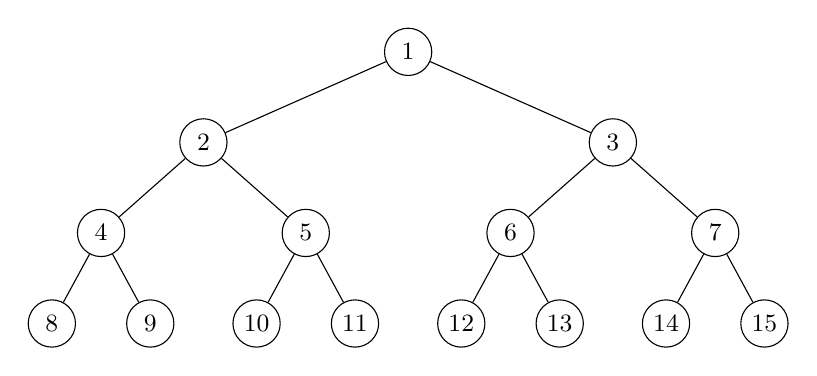
\begin{tikzpicture}[
  level distance=1.15cm,
  level 1/.style={sibling distance=5.2cm},
  level 2/.style={sibling distance=2.6cm},
  level 3/.style={sibling distance=1.25cm},
  every node/.style={circle, draw, inner sep=1.5pt, minimum size=6mm, font=\small}
]
\node {1}
  child { node {2}
    child { node {4}
      child { node {8} }
      child { node {9} }
    }
    child { node {5}
      child { node {10} }
      child { node {11} }
    }
  }
  child { node {3}
    child { node {6}
      child { node {12} }
      child { node {13} }
    }
    child { node {7}
      child { node {14} }
      child { node {15} }
    }
  };
\end{tikzpicture}
\end{center}

\noindent The network has $L = 14$ links.\mk{1}

\noindent Being a connected network with $N = 15$ nodes and $L = N - 1$ links it is therefore a tree.\mk{2}

\subsection*{(b)}

\noindent Degree sequence (non-increasing):
\[
  \{2, 3, 3, 3, 3, 3, 3, 1, 1, 1, 1, 1, 1, 1, 1\}.
\]
There are eight leaves (nodes $8, 9, 10, 11, 12, 13, 14, 15$), so $p_1 = 8/15$; only the root has degree $2$, so $p_2 = 1/15$; the six internal nodes $2,3,4,5,6,7$ have degree $3$, so $p_3 = 6/15$.\mk{2}

\[
  p_k =
  \begin{cases}
    8/15 & \text{for } k = 1, \\
    1/15 & \text{for } k = 2, \\
    6/15 & \text{for } k = 3, \\
    0    & \text{otherwise.}
  \end{cases}
\]
\noindent\mbox{}\hfill{\small[3]}

\noindent Average degree:
\[
  \langle k \rangle = \frac{2L}{N} = \frac{28}{15},
  \qquad
  \langle k \rangle = \sum_{k=0}^{\infty} k\, p_k
  = 1 \cdot \frac{8}{15} + 2 \cdot \frac{1}{15} + 3 \cdot \frac{6}{15}
  = \frac{28}{15}.
\]
\noindent\mbox{}\hfill{\small[2]}

\subsection*{(c)}

\noindent The diameter of the network is $D = 6$. In fact, the largest distance between two nodes in the graph is equal to $D = 6$, since, for instance, node $8$ and node $15$ are both at distance $3$ from node $1$, and given that there is only one path connecting $8$ to $15$ (remember that in a tree there exists exactly one path among each pair of nodes), that path has to pass by node $1$, and its length will be equal to $3 + 3 = 6$.\mk{3}

\noindent The set of nodes which are at distance equal to $D = 6$ is the Cartesian product of the two sets $V_1 = \{8, 9, 10, 11\}$ and $V_2 = \{12, 13, 14, 15\}$.\mk{3}

\subsection*{(d)}

\noindent In a tree there is only one shortest path between any ordered pair $(r,s)$, so with the convention used in the problem sheet the betweenness can be written as
\[
  b_i = \sum_{r=1}^{N} \sum_{s=1}^{N} n_{rs}^{i},
\]
where $n_{rs}^{i} = 1$ if the (unique) shortest path from $r$ to $s$ passes through $i$, and $n_{rs}^{i} = 0$ otherwise.\mk{3}

\noindent We denote the numerical values below by $c_i^{B}$. Paths that start or end at $i$ contribute $2N - 1 = 29$ to every node.

\medskip
\noindent\textbf{Node $1$.}
Two sub-trees (rooted at $2$ and $3$) each have $7$ nodes; every directed path from one sub-tree to the other uses node $1$, giving $2 \times 7 \times 7 = 98$ contributions. Hence
\[
  c_1^{B} = 2 \times 49 + 29 = 127.
\]
\noindent\mbox{}\hfill{\small[2]}

\noindent\textbf{Nodes $2$ and $3$.}
By symmetry, $c_2^{B} = c_3^{B}$. Node $2$ lies on all paths between the $6$ nodes in its own sub-tree (excluding $2$) and the $8$ remaining nodes, and also between the two branches $\{4,8,9\}$ and $\{5,10,11\}$:
\[
  c_2^{B} = c_3^{B} = 2 \times [(6 \times 8) + 3 \times 3] + 29 = 2 \times 57 + 29 = 143.
\]
\noindent\mbox{}\hfill{\small[2]}

\noindent\textbf{Nodes $4,5,6,7$.}
Similarly,
\[
  c_4^{B} = c_5^{B} = c_6^{B} = c_7^{B} = 2 \times [2 \times 12 + 1 \times 1] + 29 = 2 \times 25 + 29 = 79.
\]
\noindent\mbox{}\hfill{\small[2]}

\noindent\textbf{Leaves $8,9,\ldots,15$.}
Each leaf only contributes the $2N - 1 = 29$ self/endpoint paths:
\[
  c_8^{B} = \cdots = c_{15}^{B} = 29.
\]
\noindent\mbox{}\hfill{\small[2]}

\subsection*{(e)}

\noindent Largest betweenness centrality: nodes $2$ and $3$.\mk{2}

\noindent Largest closeness centrality: node $1$. For example, summing distances to all other nodes,
\[
  d_1 = 2 \cdot 1 + 4 \cdot 2 + 8 \cdot 3 = 34,
  \qquad
  d_2 = 3 \cdot 1 + 5 \cdot 2 + 2 \cdot 3 + 4 \cdot 4 = 35,
\]
so $d_1 < d_2$.\mk{5}

\noindent Largest degree centrality: the six nodes $2, 3, 4, 5, 6, 7$.\mk{2}

\subsection*{(f)}

\noindent E.g.\ adding link $(2,3)$ or link $(4,5)$ will create a triangle in the network $G'$.\mk{2}

\noindent E.g.\ adding link $(2,6)$ will create a cycle of length $4$.\mk{2}

\noindent E.g.\ adding link $(5,6)$ will create a cycle of length $5$.\mk{2}

\noindent To create a cycle of length $\ell = 7$ in the network $G'$ we need to add a link between a node in $V_1 = \{8, 9, 10, 11\}$ and a node in $V_2 = \{12, 13, 14, 15\}$. We thus have $16$ different possibilities.\mk{4}

\end{document}
